\documentclass[aspectratio=169,10pt]{beamer}
\usetheme{default}
\usecolortheme{seagull}
\setbeamertemplate{navigation symbols}{}
\setbeamertemplate{footline}[frame number]

\usepackage[utf8]{inputenc}
\usepackage[T1]{fontenc}
\usepackage{graphicx}
\usepackage{booktabs}
\usepackage{xcolor}
\usepackage{tikz}

\title{MLPC 2026 Challenge:\\Segment-Based SED in Domestic Recordings}
\subtitle{Validated Encoders}
\author{Amr Abdullah \and Ibrahim Muhammad}
\date{}

\begin{document}

% ============ Slide 0 — Title ============
\begin{frame}
  \titlepage
\end{frame}

% ============ Slide 1 — Architecture ============
\begin{frame}{System Architecture}
\begin{columns}[T]
\column{0.45\textwidth}
\textbf{Pipeline:}
\begin{enumerate}\setlength\itemsep{2pt}
  \item Per-second log-mel + scalar features (960-D)
  \item One \texttt{HistGradientBoosting} per class (drop-in
        for the baseline's per-class decision tree)
  \item Per-class threshold $\tau_c$ tuned on local val
  \item Median filter over time (window $w$)
  \item Onset/offset merging $\to$ submission CSV
\end{enumerate}
\column{0.55\textwidth}
\centering
\begin{tikzpicture}[node distance=8mm, every node/.style={font=\scriptsize}]
\node[draw, rounded corners, fill=blue!8, minimum width=2.6cm, minimum height=0.6cm] (a) {1\,s segments (960-D)};
\node[draw, rounded corners, fill=blue!12, below=of a, minimum width=2.6cm, minimum height=0.6cm] (b) {HistGB $\times$ 15};
\node[draw, rounded corners, fill=blue!16, below=of b, minimum width=2.6cm, minimum height=0.6cm] (c) {Per-class $\tau_c$};
\node[draw, rounded corners, fill=blue!20, below=of c, minimum width=2.6cm, minimum height=0.6cm] (d) {Median filter ($w$)};
\node[draw, rounded corners, fill=green!18, below=of d, minimum width=2.6cm, minimum height=0.6cm] (e) {Onset/offset rows};
\foreach \src/\dst in {a/b, b/c, c/d, d/e}
  \draw[->] (\src) -- (\dst);
\end{tikzpicture}
\end{columns}
\vspace{4pt}
\footnotesize XGBoost not installed in environment $\Rightarrow$
\texttt{HistGradientBoostingClassifier} (sklearn-native, same family).
\end{frame}

% ============ Slide 2 — Hypothesis 1 ============
\begin{frame}{Hypothesis 1 --- Boosting beats a single tree}
\textbf{Claim:} replacing per-class \texttt{DecisionTree(max\_depth=20)} with
\texttt{HistGradientBoosting} lifts macro-F1 substantially, even before
threshold tuning.
\vspace{6pt}
\begin{itemize}\setlength\itemsep{3pt}
  \item \textbf{Baseline DT, local val:} \textcolor{red!70!black}{0.307}
  \item \textbf{HistGB (best grid), local val:} \textcolor{blue!70!black}{0.467} \;(\textbf{+0.16})
  \item Best config: \texttt{max\_iter=500, max\_leaf\_nodes=31}
        (smaller leaf budget generalizes better; \texttt{max\_iter} is
        capped by early stopping).
  \item Gain comes from boosting's ability to fit non-axis-aligned
        decision regions of the 960-D space.
\end{itemize}
\begin{center}
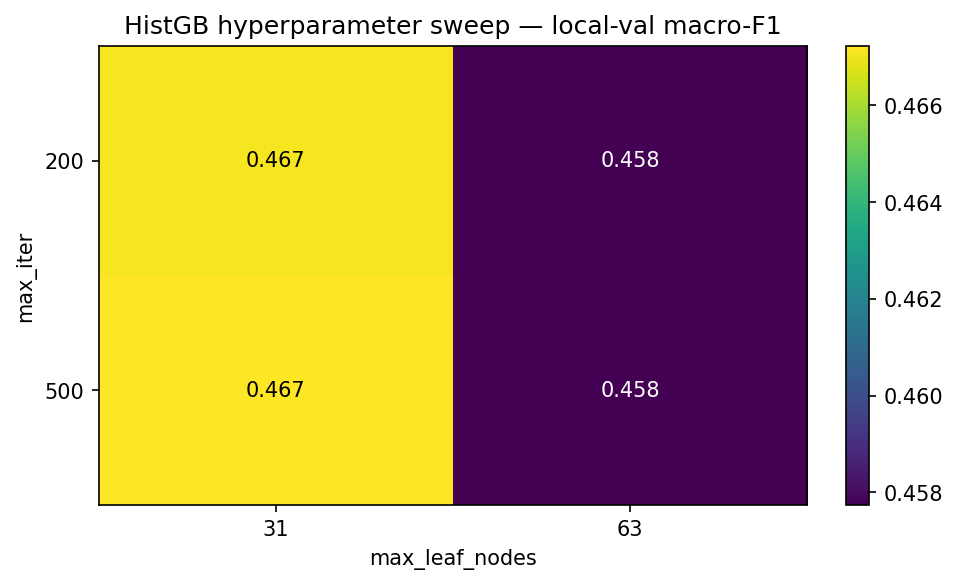
\includegraphics[width=0.7\linewidth]{../report/figures/hp_grid_heatmap.png}
\end{center}
\end{frame}

% ============ Slide 3 — Hypothesis 2 ============
\begin{frame}{Hypothesis 2 --- Per-class threshold tuning is the biggest lever}
\textbf{Claim:} the default $\tau{=}0.5$ throws away most rare-class
predictions because their posteriors sit far below 0.5.
\vspace{6pt}
\begin{itemize}\setlength\itemsep{3pt}
  \item Sweeping $\tau \in [0.05, 0.95]$ per class on local val and
        keeping the F1-optimal one lifts macro-F1 from
        \textcolor{red!70!black}{0.467} to \textcolor{blue!70!black}{0.554}
        (\textbf{+0.087}).
  \item Tuned thresholds are all low ($0.05$--$0.27$) --- rare-class
        posteriors sit far below the default $0.5$.
  \item Largest gains on rare/transient classes:
        \texttt{light\_switch}, \texttt{window\_open\_close},
        \texttt{wardrobe\_drawer\_open\_close}.
\end{itemize}
\begin{center}
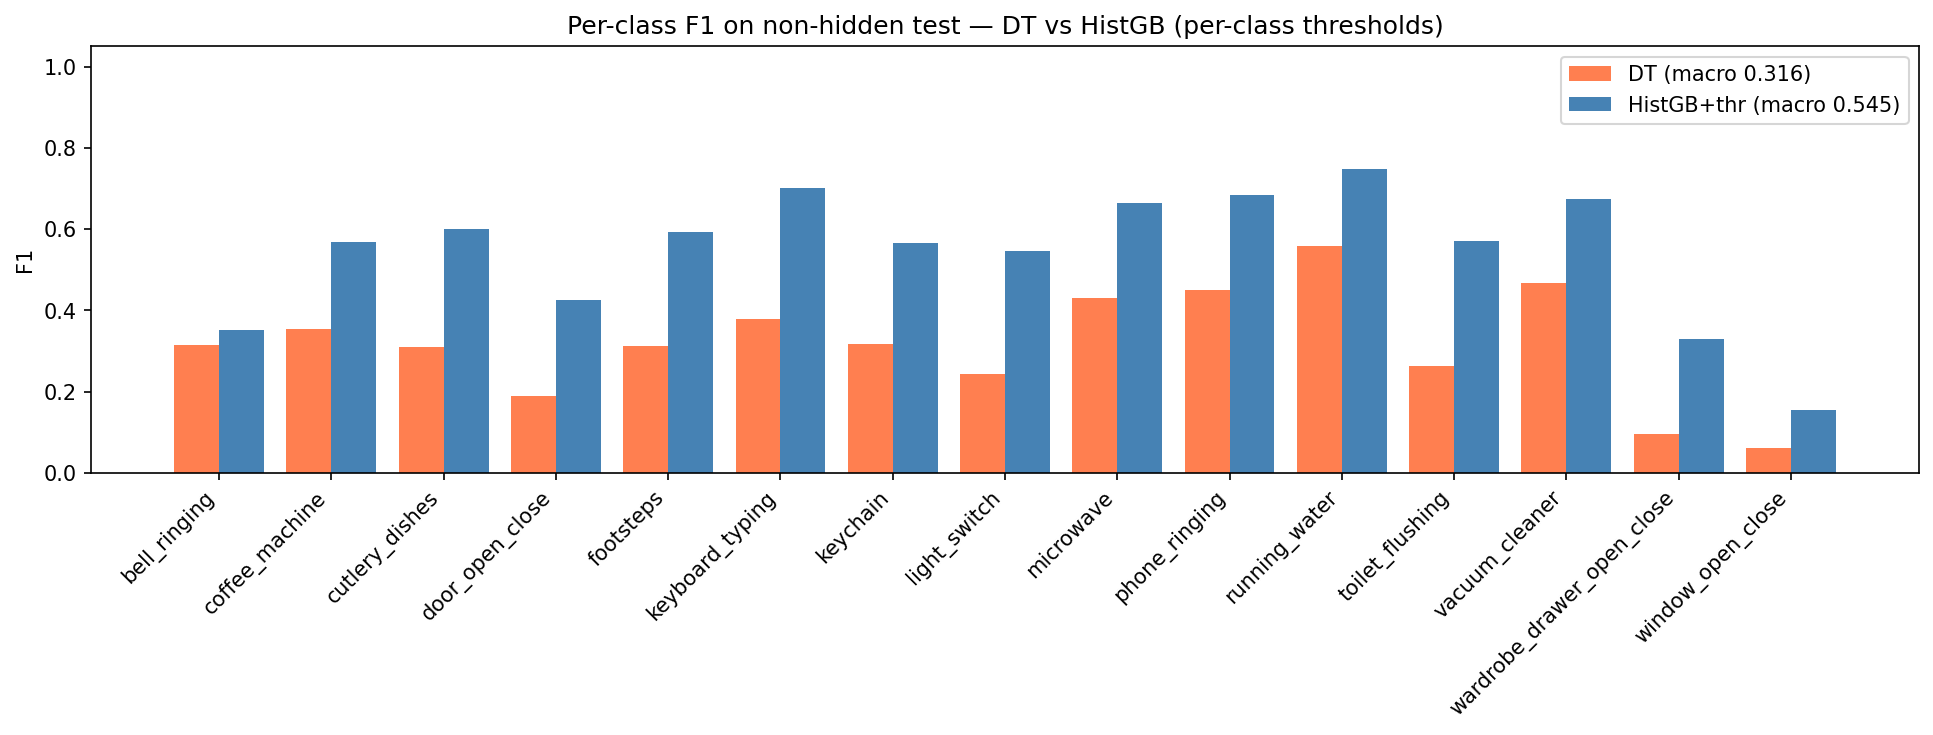
\includegraphics[width=0.95\linewidth]{../report/figures/section2_perclass.png}
\end{center}
\end{frame}

% ============ Slide 4 — Hypothesis 3 ============
\begin{frame}{Hypothesis 3 --- Median filter cleans noise but harms short events}
\textbf{Claim (refuted):} a length-$w$ median filter helps by removing
isolated false positives. \textbf{Result:} neutral --- the
threshold-tuned HistGB is already temporally coherent.
\begin{columns}
\column{0.42\textwidth}
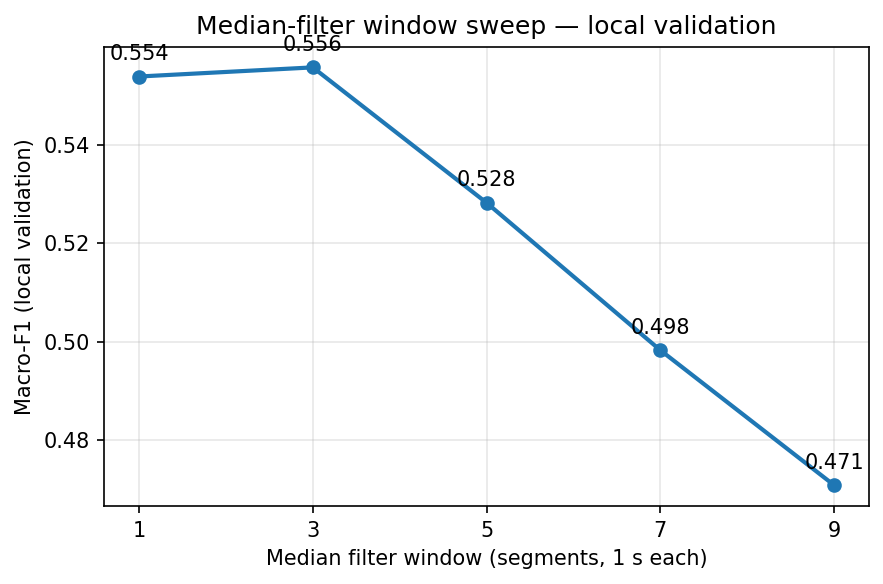
\includegraphics[width=\linewidth]{../report/figures/section3_window_sweep.png}
\column{0.58\textwidth}
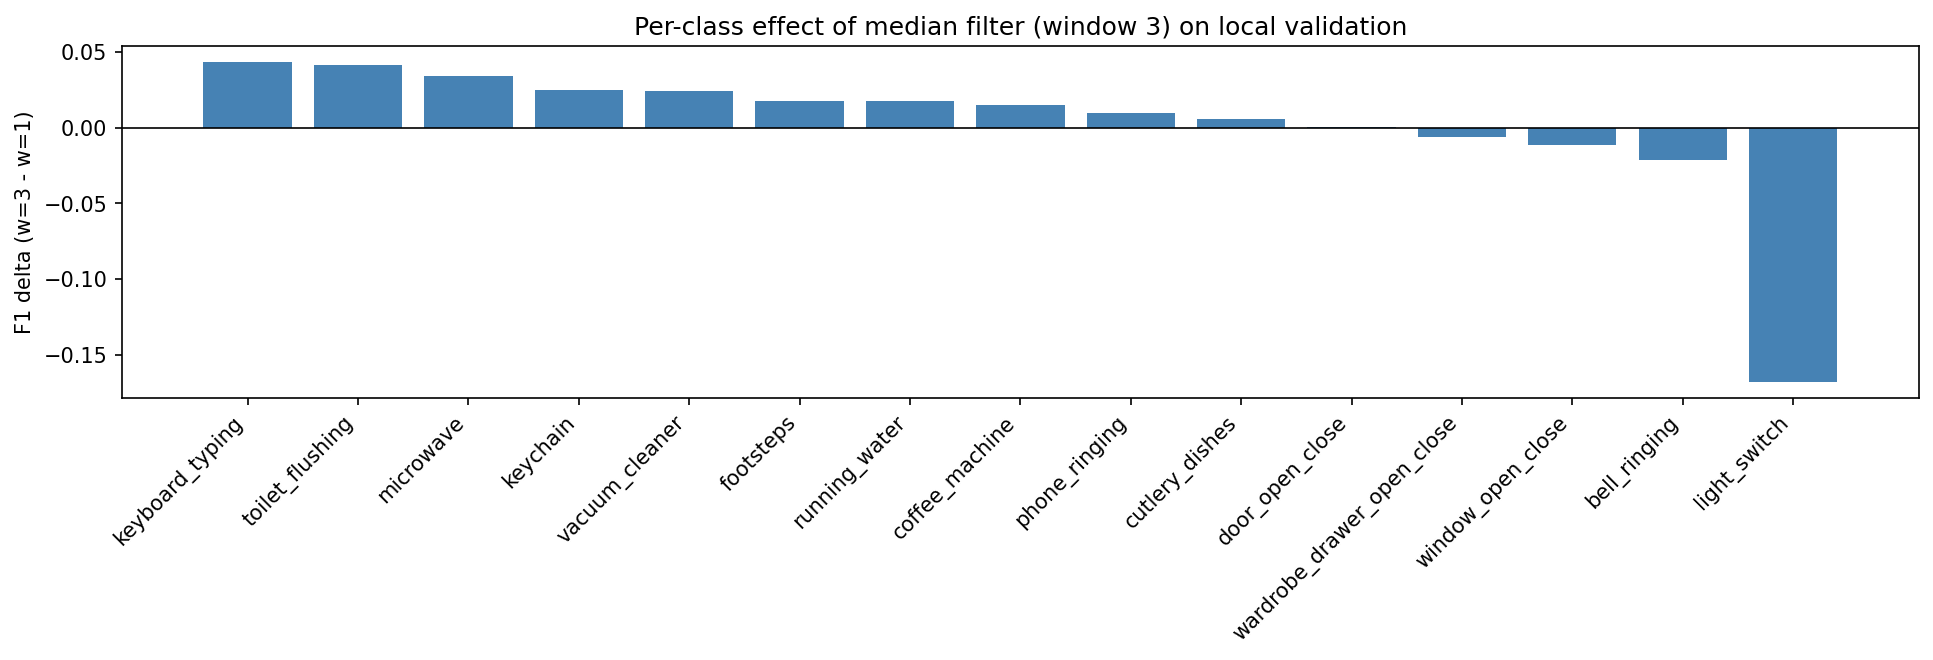
\includegraphics[width=\linewidth]{../report/figures/section3_per_class_delta.png}
\end{columns}
\vspace{2pt}
\footnotesize Best $w{=}\textbf{3}$: local-val \textbf{0.556} (no filter
\textbf{0.554}); non-hidden test \textbf{0.544} vs \textbf{0.545}
(delta \textbf{$-$0.001}). Larger $w$ erases short true events
($w{=}9$: 0.471). Remaining errors are class-confusions, not isolated
noise.
\end{frame}

% ============ Slide 5 — Failure modes / case study ============
\begin{frame}{Where the model still fails}
\begin{columns}[T]
\column{0.5\textwidth}
\textbf{Clean example} --- 3 sustained classes nailed:
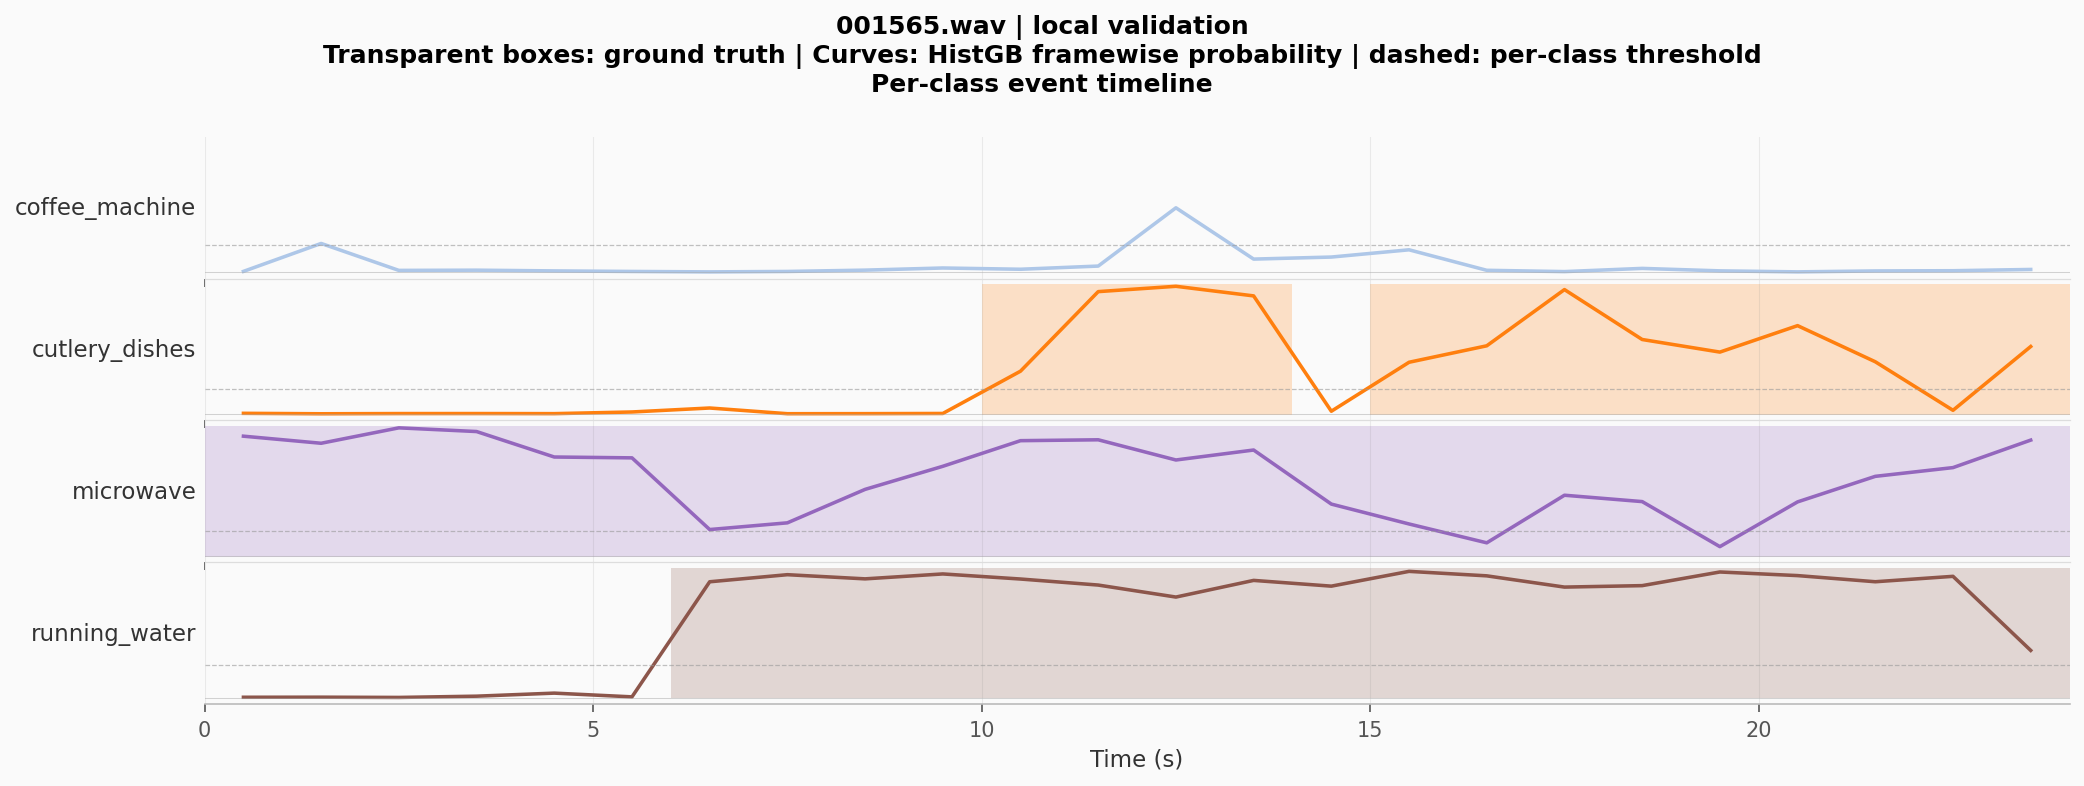
\includegraphics[width=\linewidth]{../report/figures/err_clean.png}
\column{0.5\textwidth}
\textbf{Failure example} --- model hallucinates the wrong transient:
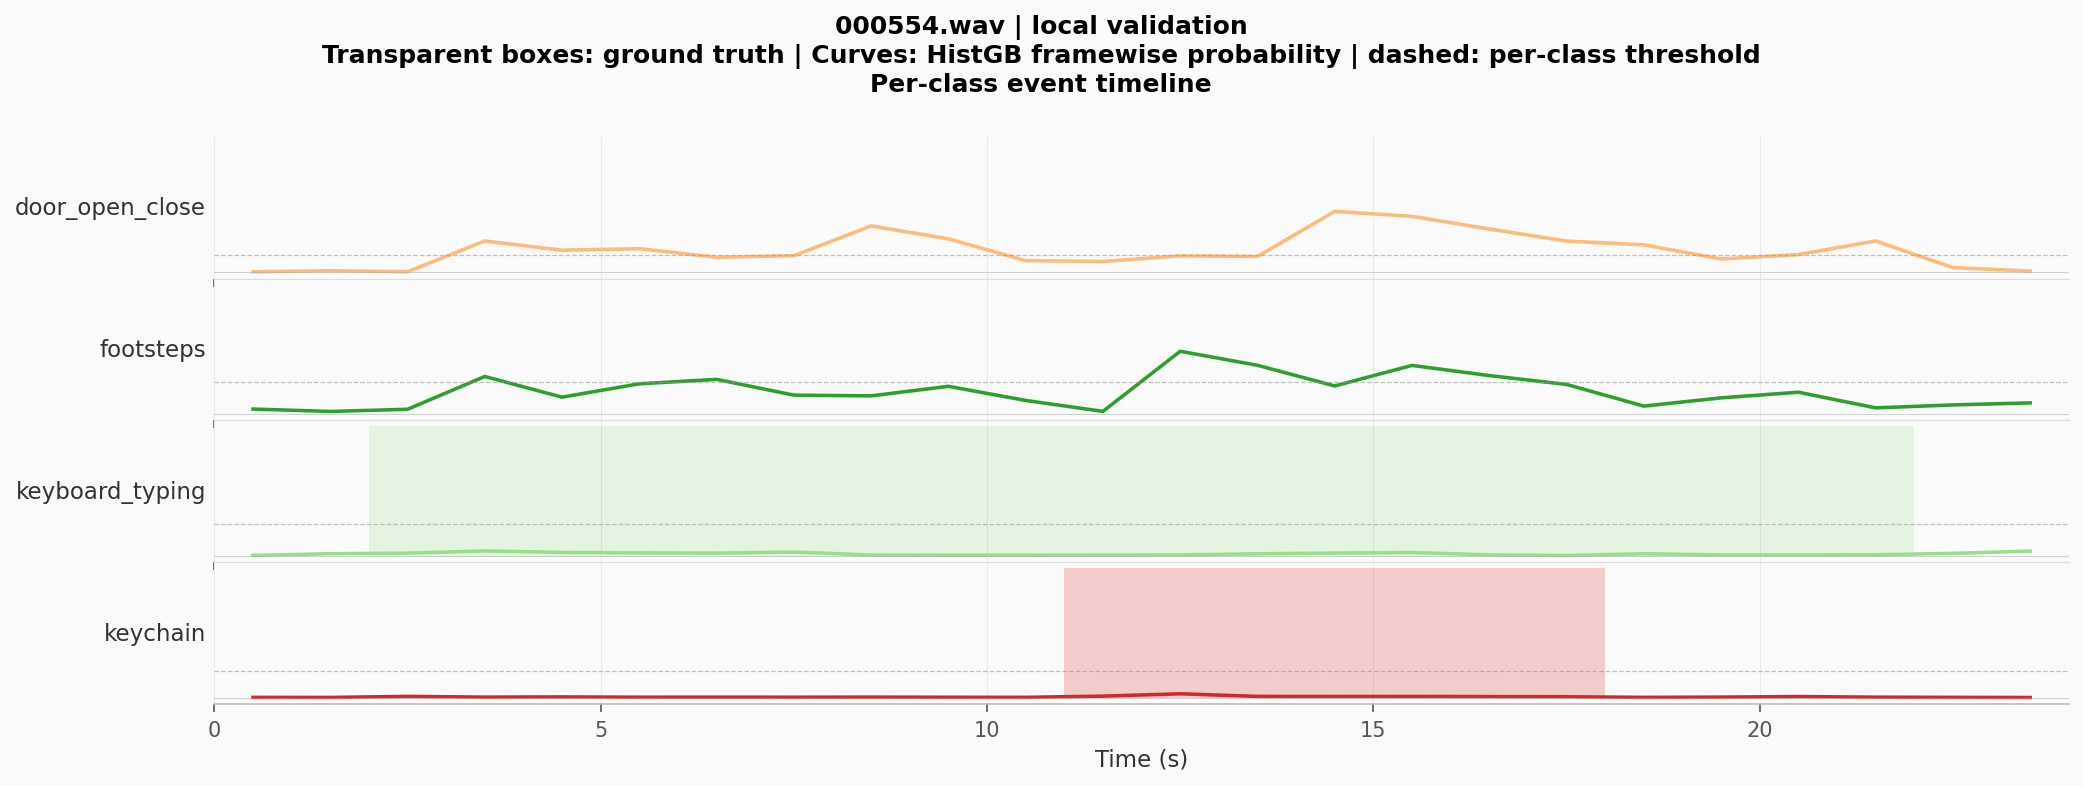
\includegraphics[width=\linewidth]{../report/figures/err_failure.png}
\end{columns}
\vspace{4pt}
\footnotesize Brief transients ($<$100\,ms) remain the dominant failure
mode: the 1\,s aggregation collapses their distinct signature.
\end{frame}

% ============ Slide 6 — Reflection + numbers ============
\begin{frame}{Summary \& Outlook}
\textbf{Final non-hidden-test macro-F1:}
\textcolor{red!60!black}{baseline DT \textbf{0.316}}
$\rightarrow$
\textcolor{blue!60!black}{HistGB + $\tau_c$ + median filter \textbf{0.544}}
\quad (\textbf{+0.228}).
\vspace{8pt}
\begin{itemize}\setlength\itemsep{4pt}
  \item Two levers did the work: \textbf{classifier swap} (DT$\to$HistGB,
        $+$0.16 on val) and \textbf{per-class threshold tuning}
        ($+$0.087 on val); post-processing was \textbf{neutral} ($\sim$0).
  \item Residual ceiling is the \textbf{1\,s temporal resolution} --- the
        shortest transient classes still score $<\!0.3$.
  \item Highest-impact next steps: (i) use the discarded half-second
        segments, (ii) move to a CRNN on raw waveforms (bonus task),
        (iii) chained classifier to capture cross-class co-occurrence.
  \item Deployment-side, the bottleneck is \textbf{threshold transfer}
        to new homes, not latency or compute.
\end{itemize}
\end{frame}

\end{document}
